\section{MNIST data experiment}
The MNIST (Modified National Institute of Standards and Technology) database comprises a collection of 60,000 training images and 10,000 testing images. These images represent handwritten digits and are digitally captured in a grayscale format, contained within a 28x28 pixel bounding box. \cite{deng2012mnist} To replicate the characteristics of the seismic traces interpolation problem, we adopted a strategy of masking 50\% of the columns in the images randomly. Subsequently, these partially masked images were fed into the generator. The generator, in turn, produced reconstructed images that effectively addressed the missing traces. 
\\\\
\noindent Three GAN architectures were utilized in this experiment. The Linear model incorporates a generator and discriminator, both constructed with the linear layer model (section \ref{sub:linear}). The LeNeT-5 model is composed of a generator using the linear layer model and a discriminator implemented with LeNeT-5 architecture (section \ref{sub:linear}). Additionally, the U-NET model integrates a generator based on U-NET and a discriminator constructed with a modified U-NET architecture (section \ref{sub:unet}).
\\\\
\noindent All three models underwent training using the Adam optimizer with a batch size of 64 and a learning rate of 0.0002. Dropout, with a probability of 0.5, was applied to both the generator and discriminator to enhance model generalization. The training ratio between the generator and discriminator was set to 2:1, emphasizing the importance of the generator's performance in image reconstruction. These parameter choices were meticulously chosen based on iterative experiments. Additional hyper-parameters for model training are detailed in the appendix table \ref{tab:param}.
\\\\
In Figure \ref{fig:mnist}, two generated samples are showcased. It is evident that the U-NET model produces results with the highest definition and bears the closest resemblance to the original images. The Linear model outputs a more generic representation of the digit along with a noisy background. The LeNeT-5 model performs between the aforementioned two models. Notably, in the example of the digit '4', both the Linear model and LeNeT-5 struggle to discern whether the masked image represents a '4' or '9', leading to a smudged reconstruction in the upper part of the image."

\begin{figure}[H]
    \centering
    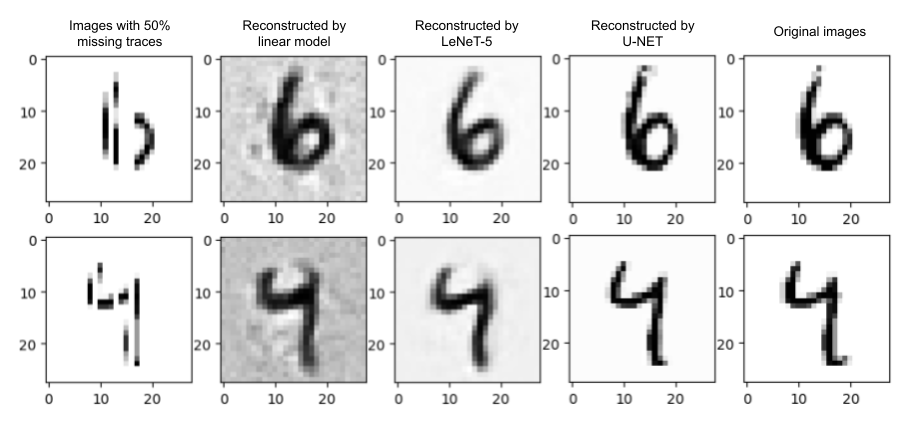
\includegraphics[width=\textwidth]{Figure/Front_page/mnist reconstruction.png}
    \caption{\textit{MNIST data reconstruction results comparison (from left to right: 50\% masked image, image reconstructed by the linear layer model, image reconstructed by LeNeT-5, image reconstructed by U-NET, original image) }}
    \label{fig:mnist}
\end{figure}

\section{F-MNIST data experiment}
Fashion-MNIST (F-MNIST) is a dataset comprised of Zalando's fashion article images. Each instance in the dataset is represented by a 28x28 pixel grayscale image, associated with a specific label from a set of 10 classes. These classes cover various fashion items, including shirts and sandals. \cite{xiao2017fashion} The dataset's size, GAN architectures, and hyper-parameters used in our experiment mirror those of the MNIST experiment. The only distinction lies in the training dataset, where Fashion-MNIST is employed.
\\\\
In Figure \ref{fig:fmnist}, the U-NET model exhibits superior performance in reconstructing intricate details of the clothing items. While LeNeT-5 demonstrates more refined edges compared to the Linear model, both models struggle to reproduce patterns on the shirt and accurately locate the straps on the sandal. Additionally, the reconstructed background in both cases appears noisy.

\begin{figure}[H]
    \centering
    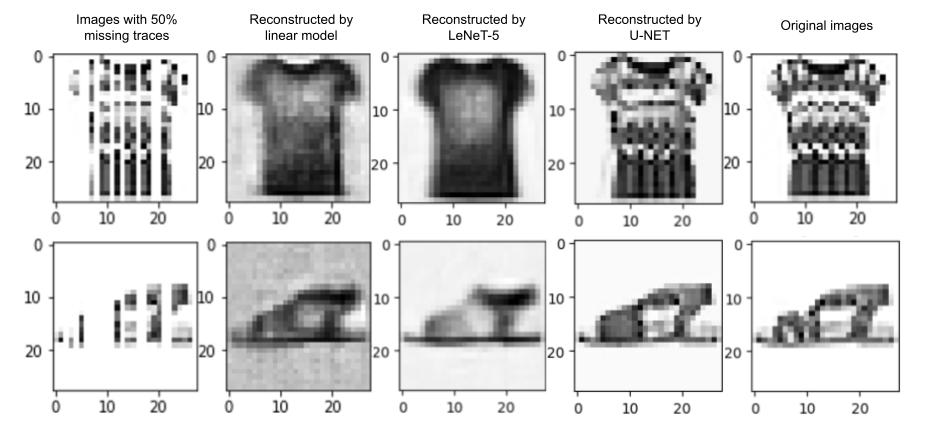
\includegraphics[width=\textwidth]{Figure/Front_page/fmnist reconstruction.png}
    \caption{\textit{Fashion-MNIST data reconstruction results comparison (from left to right: 50\% masked image, image reconstructed by the linear layer model, image reconstructed by LeNeT-5, image reconstructed by U-NET, original image)}}
    \label{fig:fmnist}
\end{figure}

\section{Discussion}
In Figures \ref{fig:mnist} and \ref{fig:fmnist}, we qualitatively assess the image reconstruction results. For a quantitative analysis, we examine the average loss per epoch of the GANs. The average discriminator losses converge to a value of 0.693, indicating that the generator produces replicas close enough to the original dataset to confuse the discriminator, i.e., the discriminator gives a guess of 0.5 for the input images. Substituting $D(x_{D}) = 0.5$ and $D(x_{G}) = 0.5$ into Equation \ref{eq:loss_D} yields a result of 0.693.
\\\\
The discriminator loss incorporates two binary cross-entropy (BCE) losses (equation \ref{eq:loss_D}), while the generator loss combines BCE loss and mean squared error (MSE) loss (equation \ref{eq:loss_G}). BCE losses are interdependent on the generator and discriminator within a model. To quantitatively evaluate the reconstruction results across models, we focus on the average generator MSE loss between the reconstructed and original images. 
\\\\
\noindent The training loss data indicates the models are well trained by the third epoch. (Figure \ref{fig:loss}) In the final epoch of MNIST validation, the average MSE losses are 0.0064, 0.0150, and 0.0213 for U-NET, LeNeT-5, and the Linear model, respectively. For F-MNIST training, the average MSE losses are 0.0065, 0.0162, and 0.0140. Excluding the Linear model, the average MSE loss is lower for the MNIST dataset, as handwritten digits contain fewer details than fashion items. U-NET outperforms the LeNeT-5 model by approximately 2.5 times. It's noteworthy that the computation time of U-NET is five times longer than LeNeT-5, with 7.18 seconds/iteration and 1.29 seconds/iteration, respectively, due to the increased complexity of the U-NET architecture. 
\\\\
\noindent The U-NET generator exhibits greater parameter efficiency, featuring 1,864,002 parameters compared to the Linear model generator's 14,631,184. Despite having an order of magnitude fewer parameters, the U-NET yields significantly superior results. This underscores that the linear model contains a considerable number of unnecessary parameters.
\\\\
\begin{figure}[H]
    \centering
    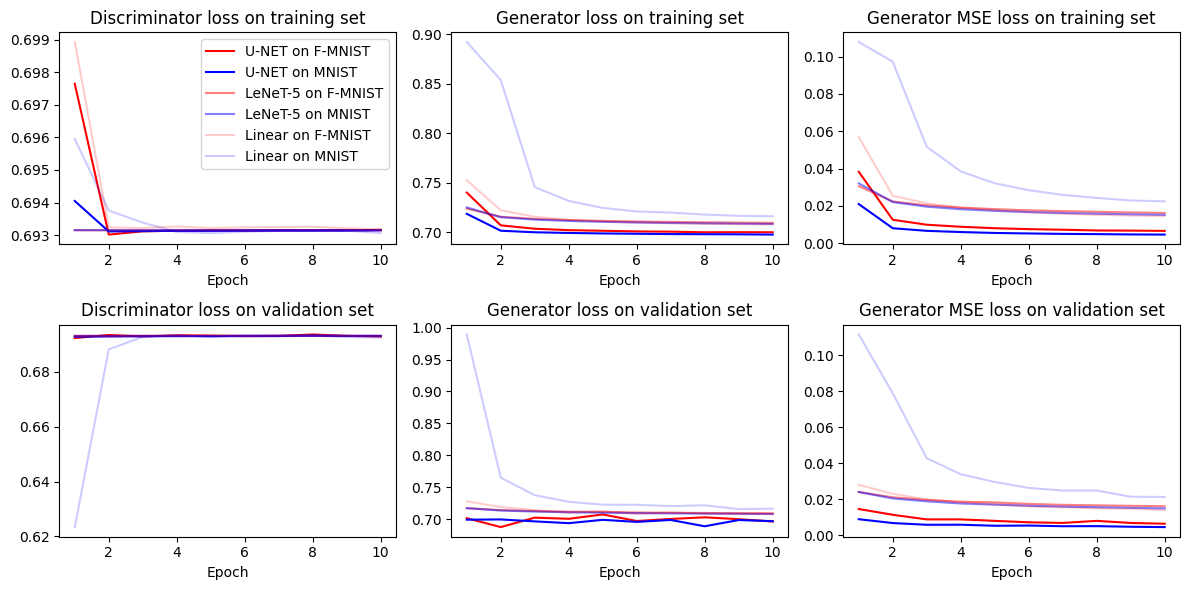
\includegraphics[width=\textwidth]{Figure/Front_page/losses.png}
    \caption{\textit{Average discriminator loss, generator loss, and generator MSE loss throughout 10 epochs for the three models on the MNIST and F-MNIST dataset}}
    \label{fig:loss}
\end{figure}

\noindent While GANs demonstrate satisfactory image reconstruction results, they are not without limitations. The first limitation is the challenge of training instability. Striking the right balance between the generator and discriminator poses difficulties, and GANs may experience oscillations or fail to converge during training. \cite{saxena2021generative} We raised the generator-discriminator training ratio to 2:1 to overcome this challenge. Second, there is the issue of feature loss due to missing information. The application of a masking function to random columns of the masked image can lead to areas with extended missing information, resulting in a blurred outcome (illustrated by the orange area in Figure \ref{fig:feature loss}). Third, GANs may encounter challenges in recovering high-frequency details. The struggle to capture intricate features, especially in small objects or complex patterns, can lead to potential smudging or loss of fine details during reconstruction (depicted by the red area in Figure \ref{fig:feature loss}).

% limitation
\begin{figure}[H]
    \centering
    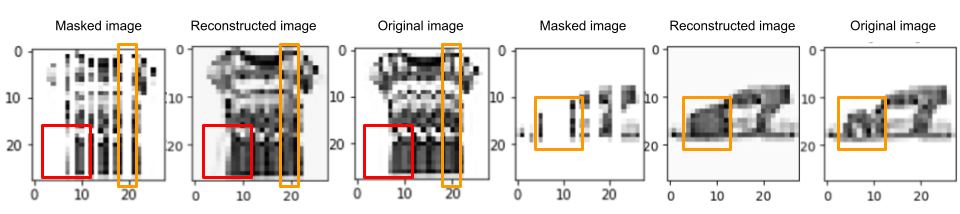
\includegraphics[width=\textwidth]{Figure/Front_page/feature lost.png}
    \caption{\textit{Feature loss in the reconstructed image due to missing information (orange) and high-frequency details (red)}}
    \label{fig:feature loss}
\end{figure}


